\chapter{Grundlagen}

Zu Beginn dieser Arbeit sollen in diesem Kapitel die dem Thema zugrunde liegenden Technologien eingegangen werden, um im Verlauf dieser Arbeit auf dieses Grundverständnis aufbauen zu können.

Zunächst soll auf die technische Basis  eines \ac{NFT}, die Blockchain und die dahinter stehende Distributed-Ledger-Technologie eingegangen werden und die Funktionsweise erläutert werden.
Darauf aufbauend werden Smart Contracts beleuchtet da sie die Implementierung eines NFTs erst ermöglichen.

\section{Blockchain und Distributed-Ledger-Technologie}

Der Begriff Blockchain stammt aus dem Kontext der, oft als Synonym verwendeten, Distributed-Ledger-Technologie, kurz DLT \parencite[vgl.][5]{WILKENS.2019}.

\subsection{Distributed-Ledger-Technologie}

Ins Deutsche übersetzt heißt Distributed Ledger so viel wie verteiltes Kontobuch und bezeichnet eine Netzwerkstruktur in der Daten verteilt organisiert sind (Abb. \ref*{fig:network} rechts).
Die Transaktionshistorie und andere Daten werden bei allen Netzwerkteilnehmern gleichzeitig gespeichert und mithilfe eines Konsensverfahrens verifiziert.
Anders als bei gewöhnlichen Datenbanken (Abb. \ref{fig:network} links) werden die Daten beim \ac{DLT} also weder zentral gespeichert, noch gibt es eine Autorität (Abb. \ref{fig:network} Mitte) welche die Daten verwaltet
\parencite[vgl.][4]{janaessebier.2017}.

    \begin{figure}
        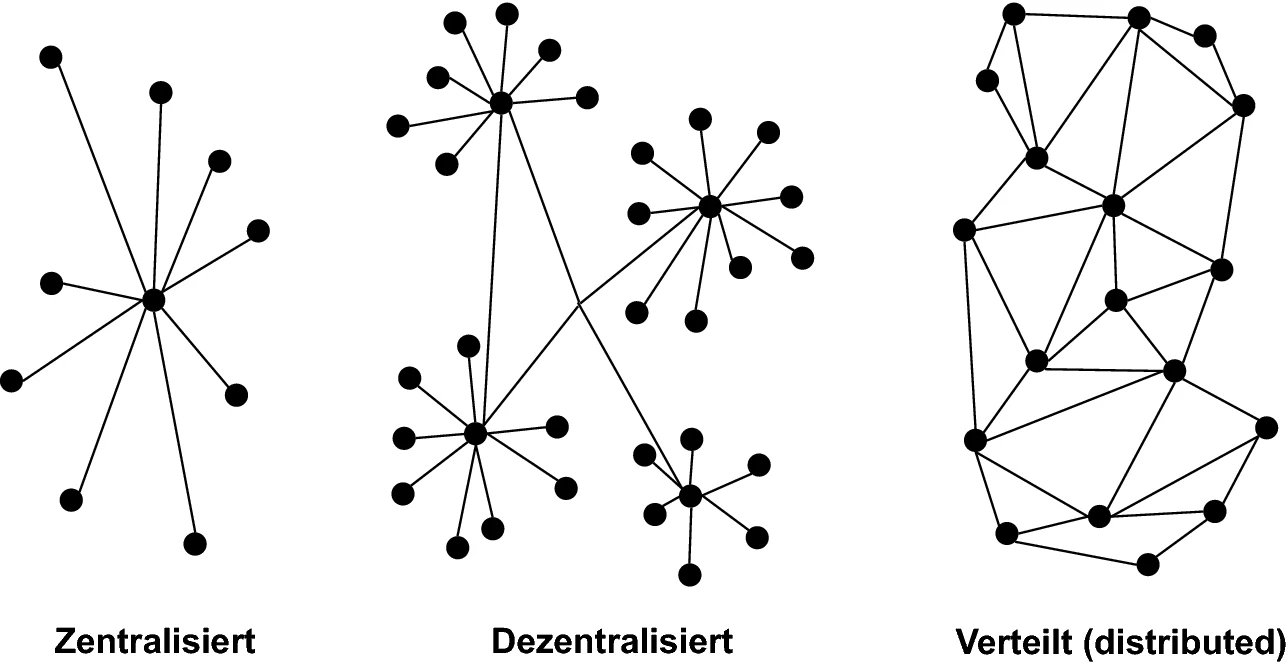
\includegraphics[width=10cm]{Bilder/Netzwerk2 (convert.io).png}
        \centering
        \captionabove[Netzwerktypen]{Netzwerktypen \parencite[vgl.][6]{WILKENS.2019}}
        \label{fig:network}
    \end{figure}

Durch die Verteilung von Datenpflege und transparenter Verwaltung durch eine große Anzahl an Nutzern im Netzwerk sind Daten fälschungssicher und nachvollziehbar.
Ein weiterer Vorteil ist die Unabhängigkeit des Netzwerks vom einzelnen Nutzer, wodurch das System sehr stabil und nahezu ausfallsicher ist \parencite[vgl.][3]{Overcamp.2019}.

\subsection{Blockchain}

Blockchains sind die derzeit bekannteste Ausprägung der \ac{DLT} und spätestens seit der Einführung von Bitcoin sollte jeder diesen Begriff schonmal gehört haben. Aber was ist das besondere an der Technologie?

Die Besonderheit der Blockchain ist die irreversible Speicherung von Transaktionen wie beispielsweise die Überweisung einer Kryptowährung, die Registrierung eines Dokuments oder Vertrags in Form aneinander hängender Blöcke. 

Dafür werden zuerst die zu übermittelnden Transaktionen beim Sender codiert. 
Dann werden die Zeichenfolgen in eine uniforme Codierungen überführt \parencite[vgl.][313]{Neugebauer.2018}.
Diese ist stark kollisionsfrei, es ist also schwer aus verschiedenen Eingaben denselben Wert abzubilden \parencite[vgl.][]{tuchemblockchain}.
Ist die Transaktion dann vom Sender an das Netzwerk übergeben worden und an die Knoten verteilt, beginnt die Prüfung der Transaktion.
Nach einer formalen Prüfung versuchen die Knoten, auch Miner genannt, durch verschiedenste Verfahren wie beispielsweise \ac{PoW} oder \ac{PoS} einen Konsens zu finden.
Zu erläutern wie diese Konsensverfahren funktionieren würde den Rahmen an dieser Arbeit jedoch sprengen. 
Ist der Konsens gefunden, ist die Transaktion validiert und wird mit anderen Transaktionen in einem Block gespeichert.
Dieser Block wird wiederum durch Hashfunktionen in ein standardisiertes Format gebracht und hierarchisch verdichtet.
In den Hashwert ist unter anderem eine Referenz auf den Hashwert des vorigen Blocks integriert, wodurch eine irreversible Verkettung der einzelnen Blöcke entsteht -- die Blockchain.
Das macht die Blockchain-Technologie gegen Manipulationsversuche sicher, weil bereits die Änderung einer einzelnen Transaktion den Hashwert
des gesamten Blocks ändern und damit die Konsistenz des Hash-Baums aufheben würde \parencite[vgl.][313]{Neugebauer.2018}.

    \begin{quote}
        „Diese hierarchische Verdichtung wird als Hash- oder Merkle-Baum bezeichnet, mit dem sich ein Block von Transaktionen eindeutig repräsentieren lässt.“
        \parencite[313]{Neugebauer.2018}
    \end{quote}

    \begin{figure}
        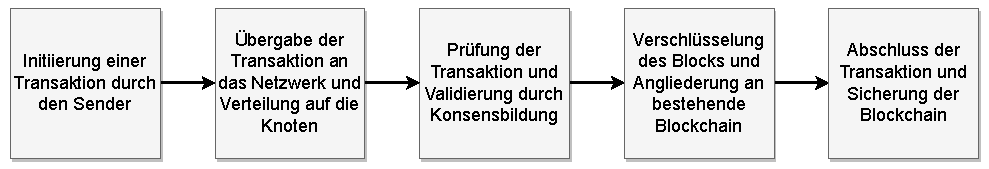
\includegraphics[width=15.8cm]{Bilder/Blockchain_schema.pdf}
        \centering
        \caption{Funktionsweise einer Blockchain}
    \end{figure}

Um die Blockchain persistent zu sichern wird die gesamte Blockchain in jedem Knoten gespeichert und bei jedem neuen Block erweitert.
Die Blockchain Technologie könnte man also als eine Art verteilte von Nutzern verwaltete Datenbank sehen.
Diese verteilte Datensicherung und -verarbeitung ist gegenüber zentralen Ansätzen deutlich weniger fehleranfällig,
bringt jedoch auch einen hohen Verbrauch an Ressourcen wie Speicherplatz und Stromverbrauch mit sich \parencite[vgl.][314]{Neugebauer.2018}.

\section{Smart Contracts}

Die Herkunft des Begriffs Smart Contract geht auf den amerikanischen Informatiker und Juristen Nick Szabo zurück,
welcher erstmals ende der 90er Jahre das Konzept rechtsrelevanter Computerprogramme und -protokolle beschrieb.

    \begin{quote} 
        „Ein Smart Contract ist eine Reihe von Zusagen, die in digitaler Form niedergelegt werden, einschließlich Protokollen, in denen die Parteien diese Zusagen einhalten.“
        \parencite[3]{WILKENS.2019}

        „[…] A smart contract is a set of promises, specifed in digital form, including protocols within which the parties perform on these promises.“
        \parencite[]{.23.01.2006}
    \end{quote}

Nick Szabo nutze für Erklärungen das Beispiel eines Warenautomats: Der Kunde wirft genügend Geld in den Automaten wählt das gewünschte Produkt und bekommt es ausgeworfen.
Im Gegenteil zum Supermarkt ist hier keine andere Person unmittelbar beteiligt und der Kauf findet automatisiert statt.
Ebenso funktionieren Smart Contracts auf digitaler Ebene, wie beispielsweise in Abbildung \ref{smartcontract} \parencite[vgl.][618]{Kaulartz.2016}:

    \begin{enumerate}
        \item Prüfbares Ereignis wird digital ausgelöst (Eingang der Transaktion)
        \item Programmcode verarbeitet das Ereignis (Prüfung der Transaktion)
        \item Handlung auf dessen Grundlage das Ereignis wird ausgeführt (Ausgabe der Ware)
    \end{enumerate}

Die Smart Contracts agieren dabei komplett automatisch und bringen damit ein hohes Potenzial für den digitalen Geschäftsverkehr mit,
da viele Prozesse automatisiert werden könnten \parencite[vgl.][27]{JohannesScherk.2017}.

Aber die Möglichkeit der Automatisierung ist nicht der alleinige Grund für die steigende Euphorie gegenüber Smart Contracts.
Die wichtigste Bedeutung entsteht in Verbindung mit der Blockchain-Technologie.
Hier können die Smart Contracts in manipulationssicheren Datenstrukturen und in redundanter Form auf allen Miner-Instanzen des Netzwerks gesichert werden.
Womit sie das komplette Gegenteil des bisher genutzten Client-Server-Modells darstellt.

Die erste Anwendung dieser Technologie ist heute allgemein hin als die Kryptowährung Bitcoin bekannt.
Durch eine Weiterentwicklung des Konzepts ist es auch möglich Programmcode in der Blockchain abzulegen und auszuführen.
Diese komplett autonomen Akteure innerhalb des Netzwerks, werden allein durch ihren Code gesteuert und ermöglichen es damit zuvor festgelegte Prozesse innerhalb der Blockchain-Umgebung automatisiert auszuführen.
Heutzutage werden mit dem Begriff Smart Contracts deshalb in aller Regel kleine Programme auf der Blockchain bezeichnet \parencite[vgl.][4]{WILKENS.2019}.
Folgende Definition wird festgehalten:

    \begin{quote}
        „Als Smart Contracts werden Programme auf der Blockchain bezeichnet, die auf Basis einer WENN-DANN-Logik arbeiten, 
        sodass bei Eintritt eines zuvor festgelegten Ereignisses (sog. Trigger)
        automatisch eine ebenfalls zuvor festgelegte Aktion (bspw. eine Transaktion) ausgeführt wird.“
        \parencite[4]{WILKENS.2019}
    \end{quote}

    \begin{figure}
        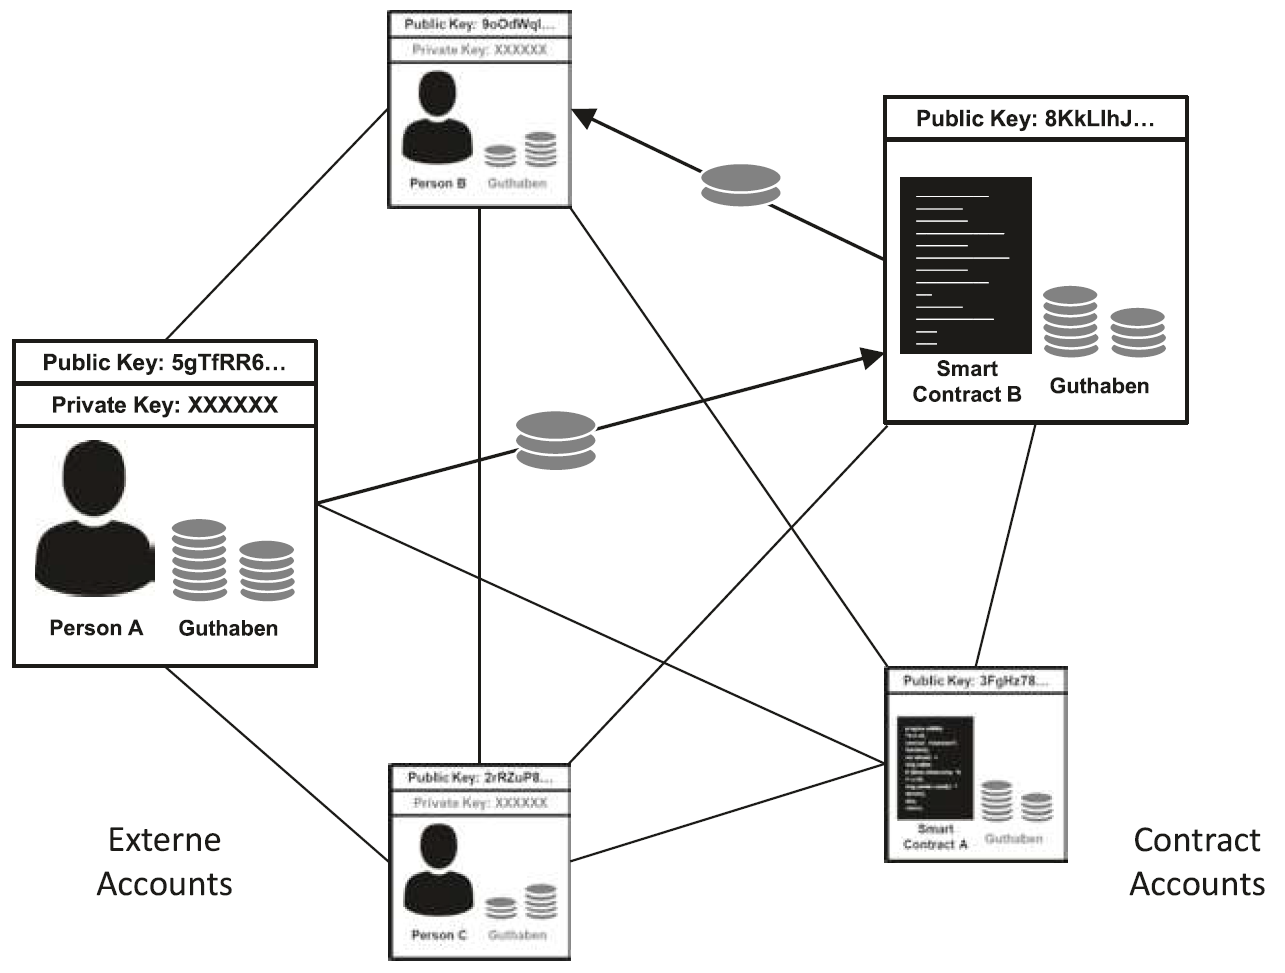
\includegraphics[width=12cm]{Bilder/Smart Contracts.PNG}
        \centering
        \captionabove[Interaktion zwischen Personen und Smart Contracts]{Interaktion zwischen Personen und Smart Contracts \parencite[vgl.][11]{WILKENS.2019}}
        \label{smartcontract}
    \end{figure}

\section{NFTs vs Kryptowährungen}

Da die technischen Grundlagen nun dargestellt wurden, soll nun erklärt werden was einen \ac{NFT} ausmacht und wo die Unterschiede zu, oft direkt im Zusammenhang genannten, Kryptowährungen bestehen.
Gemein haben \acl{NFT}s wie auch Kryptowährungen die zugrundeliegende Blockchain-Technologie und werden über Kryptobörsen veräußert.
Um die Unterschiede besser darstellen zu können wird kurz erklärt, was eine klassische Kryptowährung spezifiziert \parencite[vgl.][13]{BenjaminKraudinger.2022}.

Kryptowährungen wie beispielsweise Bitcoin, Ether (Währung der Ethereum-Blockchain) und Binance Coin sind durch zwei Charakterstika gekennzeichnet:

Zunächst wird eine Kryptowährung von Beginn an in der Blockchain implementiert.
Es ist also von Anfang an im Quellcode festgelegt welche Bezeichnung und weiteren Eigenschaften die Währung besitzt. 
Wenn sogenannte \dq Miner\dq{} also neue Einheiten erschaffen ist das eher irreführend da diese bereits im Programm vorgesehen waren und unter bestimmten Voraussetzungen freigeschaltet werden \parencite[vgl.][801]{Gassebner.2018}.
Bei Bitcoin sind das zum Beispiel maximal 21 Millionen Bitcoin \parencite[vgl.][76]{Segendorf.2014}.

Zum anderen ist der Hauptzweck von Kryptowährungen die Benutzung als Zahlungsmittel, weshalb Kryptowährungen auch als \ac{PT} bezeichnet werden \parencite[vgl.][924]{Max.2021}.
Um dies zu erreichen, dürfen sich Token zum Beispiel ein Bitcoin, nicht im Wert von einem anderen unterscheiden, im Englischen als fungibility bezeichnet \parencite[vgl.][7]{Fairfield.2021}.

Diese beiden Eigenschaften hat ein \ac{NFT} nicht. Einerseits ist ein \ac{NFT} nicht von vornherein in der Blockchain verankert,
sondern wird durch die im Grundlagenkapitel bereits erläuterten Smart Contracts an die Blockchain angefügt.
Zum anderen sollen sie nicht als Zahlungsmittel eingesetzt werden und können daher jeden beliebigen Wert annehmen.

Ein \ac{NFT} bietet die Möglichkeit auf moderne Art digitale Werteträger auf Blockchain Basis darzustellen.
Wie im Namen schon enthalten handelt es sich dabei um nicht vertretbare Token.
Besonders daran ist, dass sie einzeln vollkommen individuell sind und es prinzipiell keinen gleichen Token gibt,
letztendlich also \dq digital Einzigartig\dq{} ist \parencite[vgl.][13]{Fairfield.2021}. 

Damit bietet ein \ac{NFT} die Lösung eines bisher großen Problems im digitalen Raum:
Digitale Werte, reichend von Abbildungen von berühmten Gemälden, bis hin zu limitierten Ausrüstungsgegenständen in Computerspielen,
einem Besitzer zuordnen und zertifizieren zu können.
Denn bisher konnten diese Werte mit minimalem Aufwand verlustfrei kopiert werden,
ohne Original und Kopie im Nachhinein unterscheiden zu können. Damit ist es auch schwer möglich einen \dq wahren\dq{} Besitzer zuzuordnen \parencite[vgl.][13]{Fairfield.2021}.

Ein \ac{NFT} kann dieses Problem lösen in dem der Token ein Objekt, beispielsweise ein Kunstwerk,
auf der Blockchain repräsentiert dem eine Seltenheit zugewiesen werden soll.
Das digitale Gut wird dabei in der Regel nicht direkt in die Blockchain aufgenommen (Off-Chain \ac{NFT}).
Es enthält lediglich eine Referenz auf den Speicherort,
sowie ein Hash der Datei des Guts um die Verbindung von Gut und \ac{NFT} beweisen zu können \parencite[vgl.][23]{Fairfield.2021}.
Eine andere Möglichkeit, On-Chain \ac{NFT} genannt, sieht vor das die Datei unmittelbar in der Blockchain verankert wird.
Prinzipiell sind diese Dateien deshalb jedoch deutlich größer und je größer die auf die Blockchain zu übertragende Datenmenge,
desto höhere Transaktionsgebühren sind zu zahlen.

Wird also beispielsweise ein digitales Kunstwerk von Person A durch einen \ac{NFT} repräsentiert und an Person B verkauft,
ändert sich der Speicherort des Bildes nicht, der \ac{NFT} wechselt jedoch seinen Besitzer.
Angenommen eine dritte Person würde sich Zugang zum Speicherort des Kunstwerks verschaffen und die Datei kopieren, so wäre die Datei an sich dieselbe,
könnte jedoch als Raubkopie leicht enttarnt werden,
da in der Blockchain zu erkennen ist, dass sich das Kunstwerk erst im Besitz von A befand und dann in dem Besitz von Person B überging.
Nur Person B ist also rechtmäßiger Eigentümer des Kunstwerks und hat alleinige Verfügung.
Wie bereits beschrieben kann man diese Transaktionen im Nachhinein nicht mehr verändern oder verfälschen.
Die Blockchain kann also durch \ac{NFT} Anwendung auch zu einem Register für Besitzerstellungen sein \parencite[vgl.][567]{Hoeren.2021}.